%---------- Inleiding ---------------------------------------------------------

% TODO: Is dit voorstel gebaseerd op een paper van Research Methods die je
% vorig jaar hebt ingediend? Heb je daarbij eventueel samengewerkt met een
% andere student?
% Zo ja, haal dan de tekst hieronder uit commentaar en pas aan.

%\paragraph{Opmerking}

% Dit voorstel is gebaseerd op het onderzoeksvoorstel dat werd geschreven in het
% kader van het vak Research Methods dat ik (vorig/dit) academiejaar heb
% uitgewerkt (met medesturent VOORNAAM NAAM als mede-auteur).
% 

\section{Inleiding}%
\label{sec:inleiding}

Twintig jaar geleden was er nauwelijks sprake van Belgische wijnbouw. De laatste jaren is deze sector echter uitgegroeid tot een productieve pijler binnen onze landbouw. Volgens \textcite{FODEconomie2024} werd er in 2023 meer dan 3,4 miljoen liter wijn geproduceerd, en die groei zet zich voort. Ten opzichte van het voorgaande jaar steeg de productie met bijna dertien procent, terwijl het aantal hectaren met elf procent toenam. Daarom krijgt deze sector aandacht binnen het\textit{ Flanders AI Research Programme} (FAIR). FAIR is een consortium van onderzoeksgroepen aan Vlaamse universiteiten en onderzoekscentra, gericht op AI-onderzoek in diverse Vlaamse sectoren. Het Instituut voor Landbouw-, Visserij- en Voedingsonderzoek (ILVO) is een van deze centra. Samen met UAntwerpen werken zij aan een usecase om taken autonoom uit te voeren in wijngaarden met behulp van AI, waaronder het monitoren van de druivenkwaliteit. 

Voor dit doel wordt een reinforcement learning (RL)-algoritme ontwikkeld dat op een kleine landbouwrobot wordt geïmplementeerd. De robot heeft een arm en sensoren om druiven te meten. Om een taak autonoom uit te voeren zijn drie controlesystemen nodig: navigatiecontrole, actuatorcontrole en taakcontrole. Het RL-model moet deze controllers samenvoegen tot één geïntegreerde controller zodat de robot zelfstandig beslissingen kan nemen, afhankelijk van de situatie.

Opdat het RL-model een goede beslissing kan nemen, moet duidelijke omgevingsinformatie worden aangereikt. Er is besloten dit te doen in de vorm van een lokale 2D-kaart van de omgeving, opgesteld met Lidar- en camerasensordata. Een mogelijke methode hiervoor is het inkleuren van gekalibreerde puntenwolken met informatie uit gesegmenteerde beelden, om deze vervolgens te projecteren op een vlak parallel aan het grondvlak. Deze bachelorproef draagt bij aan de interpretatie van camerabeelden door semantische segmentatie te realiseren.

Het semantische segmentatiemodel moet in realtime de druivenranken en -trossen kunnen segmenteren. Dergelijke modellen vereisen veel rekenkracht en geheugen. Bovendien presteren ze vaak minder goed in landbouw, omdat hun architectuur niet afgestemd is op de complexiteit van natuurlijke omgevingen en vanwege het beperkte aantal (gelabelde) datasets. Dit leidt tot de hoofdonderzoeksvraag: \emph{'Hoe kan een deep learning model worden toegepast voor realtime segmentatie van druivenranken en -trossen in wijngaarden, en hoe draagt gesimuleerde data bij aan de generalisatie?'}

De volgende deelvragen worden in deze bachelorproef behandeld:
\begin{itemize}
    \setlength{\itemsep}{0pt}
    \setlength{\parskip}{0pt} 
    \item Welke uitdagingen ondervinden segmentatiemodellen bij toepassing in de landbouw en welk model is geschikt voor druivenranken en -trossen?
    \item Op welke manier dient de synthetische data te worden samengesteld om het segmentatiemodel beter te trainen?
    \item Hoe kan modeloptimalisatie plaatsvinden om segmentatie in realtime mogelijk te maken?
\end{itemize}

Het eindresultaat van de bachelorproef is een proof-of-concept van het afgestemde segmentatiemodel voor de robot, dat gewassen in de wijngaard kan segmenteren. Het model zal worden beoordeeld op efficiëntie en nauwkeurigheid.

%---------- Stand van zaken ---------------------------------------------------

\section{Literatuurstudie}%
\label{sec:literatuurstudie}

Hier beschrijf je de \emph{state-of-the-art} rondom je gekozen onderzoeksdomein, d.w.z.\ een inleidende, doorlopende tekst over het onderzoeksdomein van je bachelorproef. Je steunt daarbij heel sterk op de professionele \emph{vakliteratuur}, en niet zozeer op populariserende teksten voor een breed publiek. Wat is de huidige stand van zaken in dit domein, en wat zijn nog eventuele open vragen (die misschien de aanleiding waren tot je onderzoeksvraag!)?

Je mag de titel van deze sectie ook aanpassen (literatuurstudie, stand van zaken, enz.). Zijn er al gelijkaardige onderzoeken gevoerd? Wat concluderen ze? Wat is het verschil met jouw onderzoek?

Verwijs bij elke introductie van een term of bewering over het domein naar de vakliteratuur, bijvoorbeeld~\autocite{Hykes2013}! Denk zeker goed na welke werken je refereert en waarom.

Draag zorg voor correcte literatuurverwijzingen! Een bronvermelding hoort thuis \emph{binnen} de zin waar je je op die bron baseert, dus niet er buiten! Maak meteen een verwijzing als je gebruik maakt van een bron. Doe dit dus \emph{niet} aan het einde van een lange paragraaf. Baseer nooit teveel aansluitende tekst op eenzelfde bron.

Als je informatie over bronnen verzamelt in JabRef, zorg er dan voor dat alle nodige info aanwezig is om de bron terug te vinden (zoals uitvoerig besproken in de lessen Research Methods).

% Voor literatuurverwijzingen zijn er twee belangrijke commando's:
% \autocite{KEY} => (Auteur, jaartal) Gebruik dit als de naam van de auteur
%   geen onderdeel is van de zin.
% \textcite{KEY} => Auteur (jaartal)  Gebruik dit als de auteursnaam wel een
%   functie heeft in de zin (bv. ``Uit onderzoek door Doll & Hill (1954) bleek
%   ...'')

Je mag deze sectie nog verder onderverdelen in subsecties als dit de structuur van de tekst kan verduidelijken.

%---------- Methodologie ------------------------------------------------------
\section{Methodologie}%
\label{sec:methodologie}

De bachelorproef doorloopt een iteratief proces en richt zich op de implementatie en verfijning van het segmentatiemodel. Het proces begint met het in kaart brengen van de variatie binnen wijngaarden, waarbij relevante kenmerken worden geïdentificeerd. Vervolgens worden camerabeelden verzameld uit echte wijngaarden en data gecapteerd uit het testveld van ILVO. Daarnaast worden gesimuleerde wijngaarden opgezet om aanvullende data te genereren.

Na de dataverzameling worden evaluatiemaatstaven bepaald om de prestaties van het model te beoordelen. De modelontwikkeling begint met het selecteren van potentiële architecturen op basis van wetenschappelijke literatuur, waarna de verzamelde data wordt voorbereid. Het gekozen model wordt eerst getraind met enkel de echte data. Daarna volgt een tweede trainingsronde, waarin eerst synthetische data en vervolgens echte data worden gebruikt om het model verder te verfijnen. Beide versies van het model worden geëvalueerd.

Binnen de iteratieve cyclus ligt de nadruk op het doorvoeren van bijsturingen op basis van de evaluatie, met als doel de prestaties te verbeteren en de sim-to-real gap te verkleinen. Dit kan onder andere inhouden dat de modelarchitectuur wordt aangepast of dat de trainingsdata wordt aangevuld. Na elke bijsturing volgt een evaluatie om de impact van de aanpassingen te meten. Tot slot wordt het model geoptimaliseerd voor realtime toepassingen, waarna een finale evaluatie plaatsvindt om de nauwkeurigheid en efficiëntie onder realtime omstandigheden te bevestigen.

Voor de uitvoering kunnen tools zoals Python, PyTorch, TensorFlow, GitHub, Blender en Roboflow worden ingezet; deze lijst is niet exhaustief of definitief.

Onderstaande figuur visualiseert het verloop:
\includegraphics[width=8cm,page=3]{methodologie.png}

%---------- Verwachte resultaten ----------------------------------------------
\section{Verwacht resultaat, conclusie}%
\label{sec:verwachte_resultaten}

Uit het onderzoek wordt een bruikbaar segmentatiemodel verwacht dat kan worden ingezet op een robot, en dat in staat is om wijngaardgewassen nauwkeurig in te kleuren op camerabeelden. Evaluatiemetrics meten hoe vergelijkbaar de modelsegmentaties zijn met de handmatige annotaties. De belangrijkste metrics zijn: Intersection over Union (IoU), Dice-coëfficiënt, precisie en recall, boundary F1-score en pixelnauwkeurigheid. De efficiëntie van het model wordt gemeten op basis van de inferentietijd, modelgrootte en geheugengebruik, samen met de benodigde rekenkracht.

De volgende verwachting is dat gesynthetiseerde data een merkbaar positief effect zal hebben op de generalisatie van het model. De evaluatiemetrics van het model worden eerst berekend na training met enkel de beperkt beschikbare echte data. Deze metrics worden vervolgens vergeleken met de metrics van het model dat is getraind op zowel echte als gesynthetiseerde data. Zo kan aangetoond worden dat gesynthetiseerde data een realistisch alternatief is voor echte data van wijngaarden, die in de praktijk moeilijk te bekomen is in grote hoeveelheden.

Dankzij succesvolle segmentatie worden de gewassen in de afbeeldingen ingekleurd. Met behulp van gekalibreerde LIDAR-sensoren kunnen deze ingekleurde gewassen vervolgens ook in de gegenereerde puntwolken worden weergegeven. De 2D-projectie van deze datapunten vormt dan een kaart waarop de gewassen zijn aangeduid. Deze informatie stelt het RL-model in staat om een beter inzicht te krijgen in zijn omgeving, wat essentieel is om zijn toestand te kennen en de juiste acties te kiezen.